% =============================================================================================
% =============================================================================================
% Document class: Beamer
\documentclass[ 10pt, xcolor = dvipsnames]{beamer}
% Packages: Beamer
\usepackage{ beamerthemesplit, lmodern}
\setbeamertemplate{frametitle continuation}{}
% Packages: LaTeX
\usepackage[ linesnumbered, ruled, vlined]{algorithm2e}
\usepackage{ amsfonts, amsmath, amssymb, amsthm}
\usepackage{ color, colortbl}
\usepackage{ dsfont}
\usepackage{ float}
\usepackage{ hhline}
\usepackage{ graphicx}
\usepackage{ latexsym}
\usepackage{ mathtools, multicol, multirow}
\usepackage{ parskip, pbox, pifont}
\usepackage{ ragged2e}
\usepackage{ setspace, stmaryrd, subcaption}
\usepackage{ tabularx}
\usepackage{ wasysym}

% =============================================================================================
% Packages: LaTeX (Depth-2)
\usepackage{ epstopdf}

% =============================================================================================
% Themes, colors and styles
\hypersetup{ colorlinks, linkcolor =, urlcolor = blue, citecolor = blue}
\usetheme{Madrid}
\usecolortheme[named=Brown]{structure} 
\useinnertheme{rectangles}
\beamertemplatenavigationsymbolsempty

% =============================================================================================
% =============================================================================================
% Macros: Calculus
\newcommand{\latParDer}[2]{ \partial {#1} / \partial {#2} }
\newcommand{\latParDerD}[2]{ \partial {#1} / \partial^2 {#2} }
\newcommand{\latParDerDer}[3]{ \partial^2 {#1} / \partial {#2} \partial {#3} }
\newcommand{\parDer}[2]{ \frac{ \partial {#1} }{ \partial {#2} } }
\newcommand{\parDerD}[2]{ \frac{ \partial^2 {#1} }{ \partial {#2}^2 } }
\newcommand{\parDerDer}[3]{ \frac{ \partial^2 {#1} }{ \partial {#2} \partial {#3} } }

% Macros: Colors
\definecolor{InkscapeBlue}{HTML}{0000FF}
\newcommand{\Blue}[1]{\color{InkscapeBlue}#1}
\newcommand{\Brown}[1]{{\color{Brown}#1}}
\newcommand{\Brbf}[1]{\Brown{\textbf{#1}}}
\definecolor{InkscapeGray}{HTML}{808080}
\newcommand{\Gray}[1]{\color{InkscapeGray}#1}
\definecolor{InkscapeGreen}{HTML}{008000}
\newcommand{\Green}[1]{\color{InkscapeGreen}#1}
\definecolor{InkscapeOrange}{HTML}{FF6600}
\newcommand{\Orange}[1]{\color{InkscapeOrange}#1}
\definecolor{InkscapePurple}{HTML}{FF00FF}
\newcommand{\Purple}[1]{\color{InkscapePurple}#1}
\newcommand{\Red}[1]{\color{Red}#1}
\definecolor{InkscapeYellow}{HTML}{DCDC00}
\newcommand{\Yellow}[1]{\color{InkscapeYellow}#1}

% Macros: Graph Theory
\newcommand{\Arcs}{\mathcal{A}}
\newcommand{\Nodes}{\mathcal{N}}

% Macros: Language
\newcommand{\define}{\triangleq}
\newcommand{\done}{\hfill $\square$}
\newcommand{\eqCIRC}{\stackrel{\circ}{=}}
\newcommand{\eqSTAR}{\stackrel{*}{=}}
\renewcommand{\epsilon}{\varepsilon}
\newcommand{\eg}{\textit{e.g.,\;}}
\newcommand{\egc}{\textit{e.g.:\;}}
\newcommand{\Eg}{\textit{E.g.,\;}}
\newcommand{\Egc}{\textit{E.g.:\;}}
\newcommand{\ie}{\textit{i.e.,\;}}
\newcommand{\iec}{\textit{i.e.:\;}}
\newcommand{\Ie}{\textit{I.e.,\;}}
\newcommand{\Iec}{\textit{I.e.:\;}}
\newcommand{\QED}{\hfill $\blacksquare$}
\newcommand{\st}{\text{ s.t. }}
\newcommand{\suchthat}{\text{ s.t. }}
\newcommand{\tand}{\text{ and }}
\newcommand{\tor}{\text{ or }}
\renewcommand{\vec}[1]{{\boldsymbol{#1}}}

% Macros: Limits
\newcommand{\igti}{i \rightarrow \infty}
\newcommand{\jgti}{j \rightarrow \infty}
\newcommand{\kgti}{k \rightarrow \infty}
\newcommand{\mgti}{m \rightarrow \infty}
\newcommand{\ngti}{n \rightarrow \infty}
\newcommand{\tgti}{t \rightarrow \infty}
\newcommand{\xgti}{x \rightarrow \infty}

% Macros: Mathcal
\newcommand{\A}{\mathcal{A}}
\newcommand{\B}{\mathcal{B}}
\newcommand{\BigO}{\mathcal{O}}
\newcommand{\C}{\mathcal{C}}
\newcommand{\D}{\mathcal{D}}
\newcommand{\E}{\mathcal{E}}
\newcommand{\F}{\mathcal{F}}
\newcommand{\G}{\mathcal{G}}
\newcommand{\I}{\mathcal{I}}
\newcommand{\K}{\mathcal{K}}
\newcommand{\M}{\mathcal{M}}
\renewcommand{\P}{\mathcal{P}}
\newcommand{\R}{\mathcal{R}}
\newcommand{\T}{\mathcal{T}}
\newcommand{\U}{\mathcal{U}}
\newcommand{\V}{\mathcal{V}}
\newcommand{\W}{\mathcal{W}}
\newcommand{\X}{\mathcal{X}}

% Macros: Optimization Theory
\DeclareMathOperator*{\argmin}{arg\,min}
\DeclareMathOperator*{\argmax}{arg\,max}
\DeclareMathOperator*{\arginf}{arg\,inf}
\DeclareMathOperator*{\argsup}{arg\,sup}

% Macros: Overrides
\renewcommand{\tilde}[1]{\widetilde{#1}}

% Macros: Probability Theory
\newcommand{\cov}{\mathbb{V}}
\newcommand{\Exp}{\mathbb{E}} % Expectation
\newcommand{\convD}{\stackrel{d}{\rightarrow}} % converges in distribution
\newcommand{\eqAS}{\stackrel{a.s.}{=}} % Equal (almost surely)
\newcommand{\eqD}{\stackrel{d}{=}} % Equal (in distribution)
\newcommand{\eqIND}{\stackrel{\bot}{=}} % Equal because of independence
\newcommand{\IndFun}{\mathbb{I}} % Indicator function
\newcommand{\Indicate}[1]{ \IndFun \, \{ \, #1 \, \} } % Indicator function
\renewcommand{\Pr}{\mathbb{P}} % Probability
\newcommand{\Normal}{\mathcal{N}} % Normal random variable
\newcommand{\std}{\text{std}} % Standard deviation
\newcommand{\supp}{\text{sop}} % Support of a distribution
\newcommand{\var}{\text{var}} % Variance

% Macros: Scripts
\newcommand{\tSup}[1]{\ensuremath{^{\text{#1}}}}
\newcommand{\tSub}[1]{\ensuremath{_{\text{#1}}}}
\newcommand{\ith}{$i$\tSup{th} }
\newcommand{\iplusth}{$(i+1)$\tSup{th}}
\newcommand{\jth}{$j$\tSup{th} }
\newcommand{\jplusth}{$(j+1)$\tSup{th}}
\newcommand{\kth}{$k$\tSup{th} }
\newcommand{\lth}{$l$\tSup{th} }
\newcommand{\mth}{$m$\tSup{th} }
\newcommand{\nth}{$n$\tSup{th} }

% Macros: Sets
\newcommand{\Bin}{\mathbb{B}}
\newcommand{\Complex}{\mathbb{C}}
\renewcommand{\emptyset}{\varnothing}
\newcommand{\diam}{\text{diam}\,} % Diameter of a set
\newcommand{\fromto}[2]{ \{ \, #1, \, \dots, \, #2 \} }
\newcommand{\Nat}{\mathbb{N}} % Naturals
\newcommand{\NatO}{{\Nat}_{0}} % Naturals including zero
\newcommand{\Rationals}{\mathbb{Q}}
\renewcommand{\Re}{\mathbb{R}} % Reals
\newcommand{\ReNN}{{\Re}_{\geq 0}} % Real non-negatives
\newcommand{\ReSP}{{\Re}_{> 0}} % Real strictly positives
\newcommand{\seq}[2]{ \{ #1 \}_{#2} }
\newcommand{\setform}[2]{ \left\lbrace \; #1 \;\; \middle| \;\; #2 \; \right\rbrace } % Set of the form ...
\newcommand{\singleton}[1]{ \{ #1 \} }
\renewcommand{\subset}{\subseteq}
\renewcommand{\supset}{\supseteq}
\newcommand{\upto}[1]{ \llbracket #1 \rrbracket } % Positive integers up to ... 
\newcommand{\Z}{\mathbb{Z}} % Integers
\newcommand{\ZNN}{\mathbb{Z}_{\geq 0}} % Integers

% Macros: Set Theory (DEPTH-2)
\newcommand{\nn}{n \in \Nat} \newcommand{\nnO}{n \in \NatO}
\newcommand{\mn}{m \in \Nat} \newcommand{\mnO}{m \in \NatO}

% =============================================================================================
% =============================================================================================
\title[\'Algebra Lineal: Taller 01]{\'Algebra Lineal: \textbf{Taller 01} }
\author[L. I. Reyes Castro]{Luis I. Reyes Castro, M. Sc.}
\institute[ESPOL]{\normalsize Escuela Superior Polit\'ecnica del Litoral (ESPOL) \\ Guayaquil - Ecuador}
\date[]{\small A\~no Acad\'emico 2016 - T\'ermino I}

\renewcommand{\figurename}{Figura}
\renewcommand{\tablename}{Tabla}

\newcommand{\fullcut}{\vspace{-\baselineskip}}
\newcommand{\fullskip}{\vspace{\baselineskip}}
\newcommand{\halfcut}{\vspace{-0.5\baselineskip}}
\newcommand{\halfskip}{\vspace{0.5\baselineskip}}

\renewcommand{\vec}[1]{\mathbf{#1}}
\newcommand{\Remat}[2]{\mathbb{R}^{ #1 \times #2 }}

% =============================================================================================
% =============================================================================================
\AtBeginSection[]
{
\begin{frame}
\frametitle{Contenido del Tema}
\tableofcontents[ currentsection, sectionstyle = show/shaded, subsectionstyle = show/show/hide]
\end{frame}
}
\AtBeginSubsection[]
{
\begin{frame}
\frametitle{Contenido del Tema}
\tableofcontents[ currentsection, currentsubsection, sectionstyle = show/shaded, subsectionstyle = show/shaded/hide]
\end{frame}
}

% =============================================================================================
% =============================================================================================
\begin{document}

% =============================================================================================
\begin{frame}[noframenumbering]
\titlepage
\end{frame}

% =============================================================================================
%\begin{frame}[noframenumbering]
%\frametitle{Contenido del Tema}
%\tableofcontents[ subsectionstyle = hide]
%\end{frame}

% =============================================================================================
% =============================================================================================
\section{Estructuras de Vigas Ideales (EVIs)}

% =============================================================================================
\begin{frame}[allowframebreaks]
\frametitle{\insertsection}

\begin{figure}
\centering
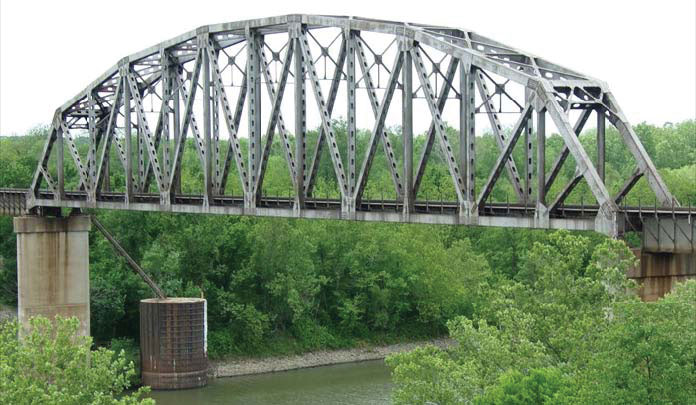
\includegraphics[ width = 0.8\textwidth]{Truss-bridge_01.jpg}
\end{figure}

\framebreak

\begin{figure}
\centering
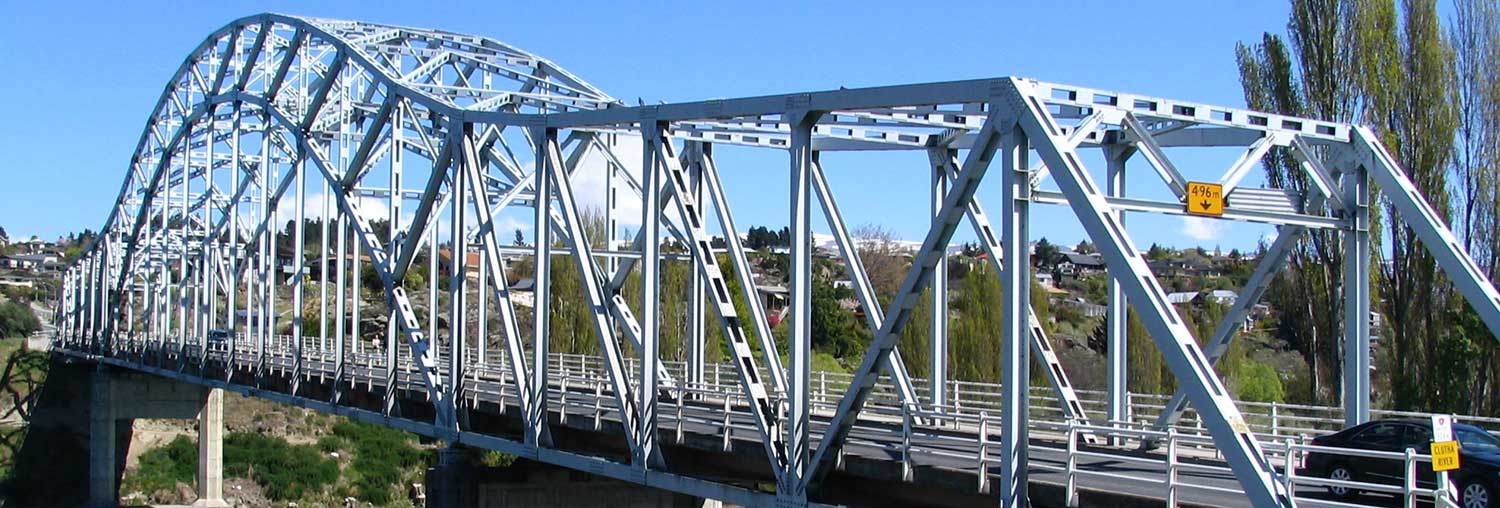
\includegraphics[ width = 0.8\textwidth]{Truss-bridge_02.jpg}
\end{figure}

\framebreak

\begin{figure}
\centering
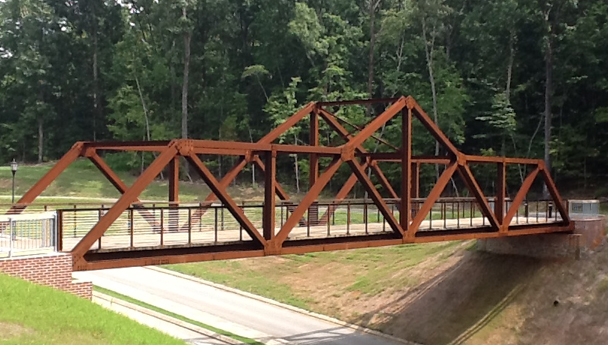
\includegraphics[ width = 0.8\textwidth]{Truss-bridge_03.jpg}
\end{figure}

\framebreak

\begin{figure}
\centering
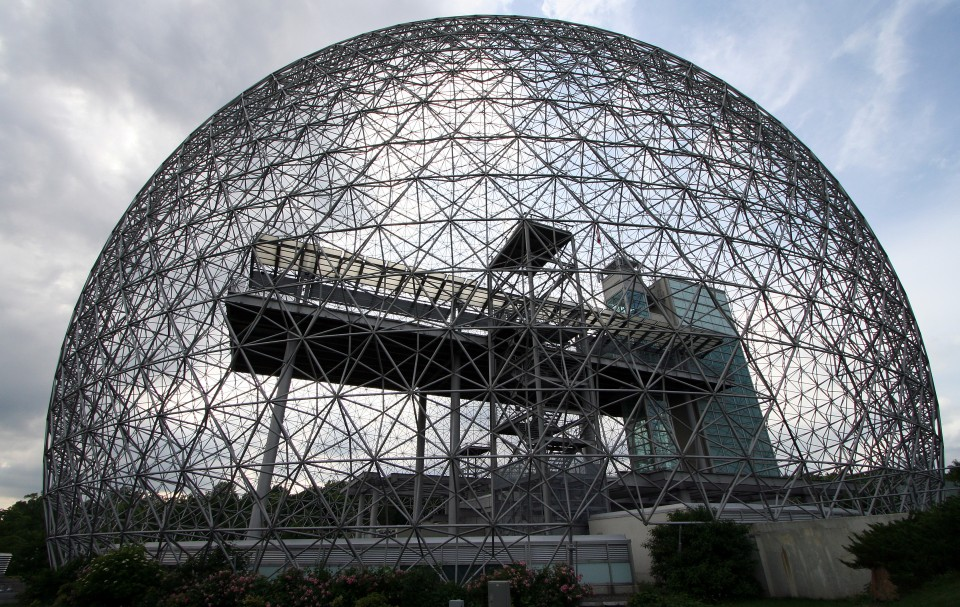
\includegraphics[ width = 0.8\textwidth]{Truss-other_00.jpg}
\end{figure}

\framebreak

\begin{figure}
\centering
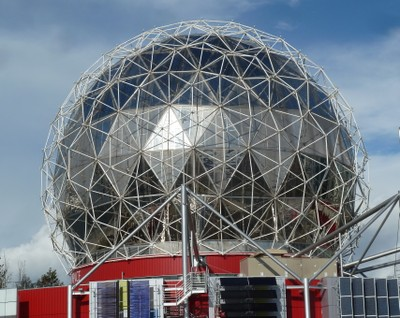
\includegraphics[ width = 0.7\textwidth]{Truss-other_01.jpg}
\end{figure}

\framebreak

\begin{figure}
\centering
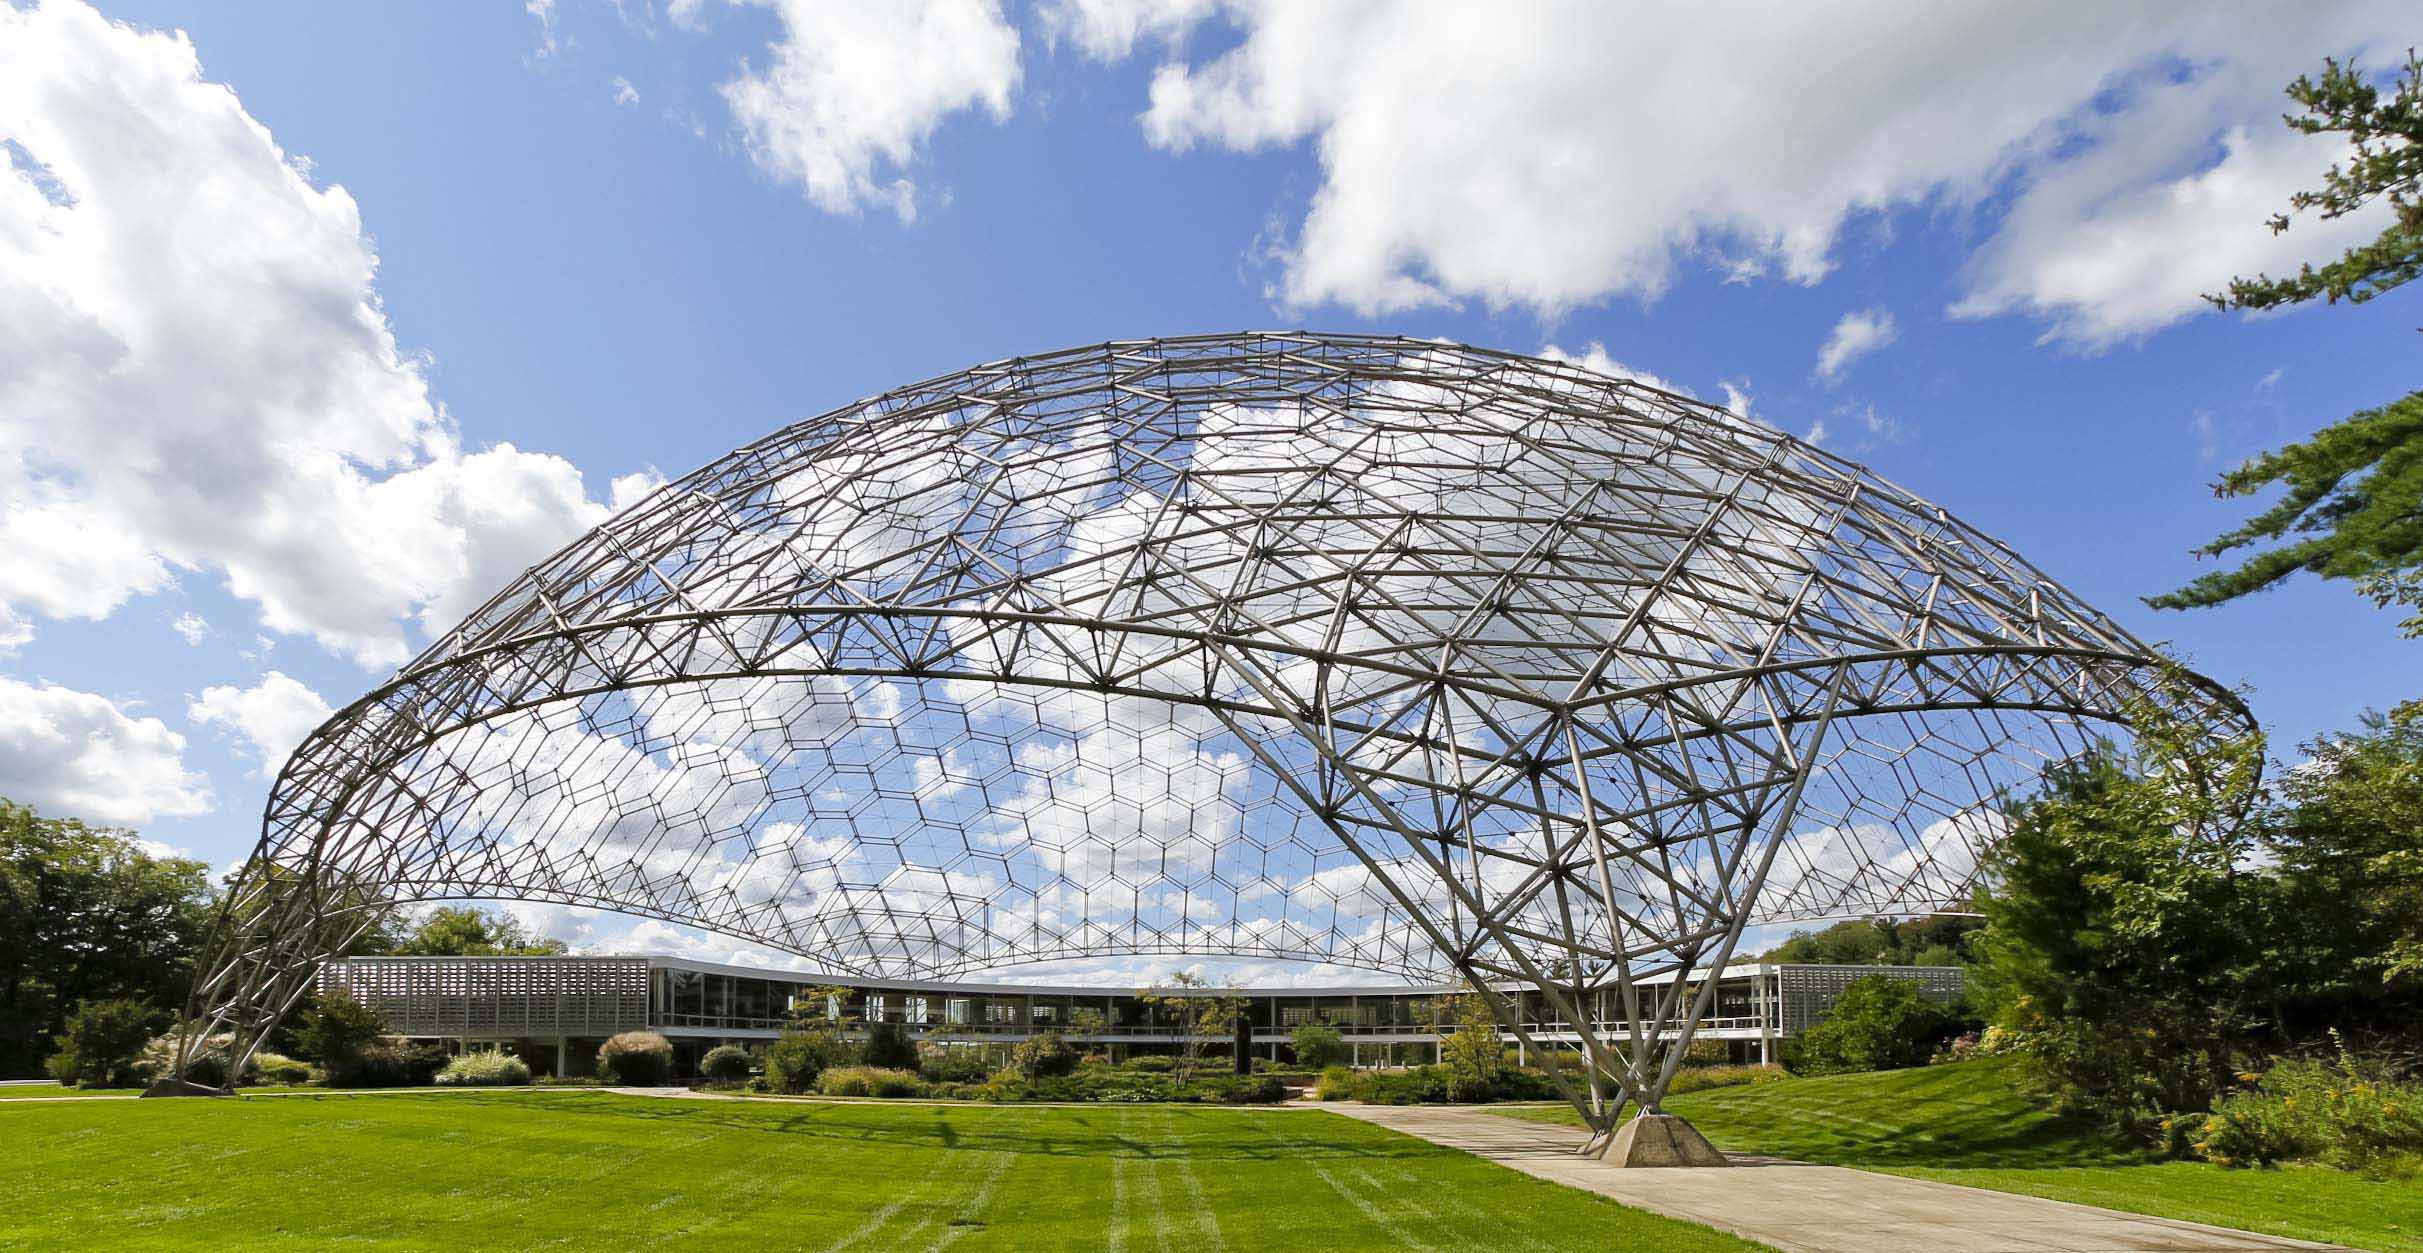
\includegraphics[ width = 0.8\textwidth]{Truss-other_04.jpg}
\end{figure}

\framebreak

\begin{figure}
\centering
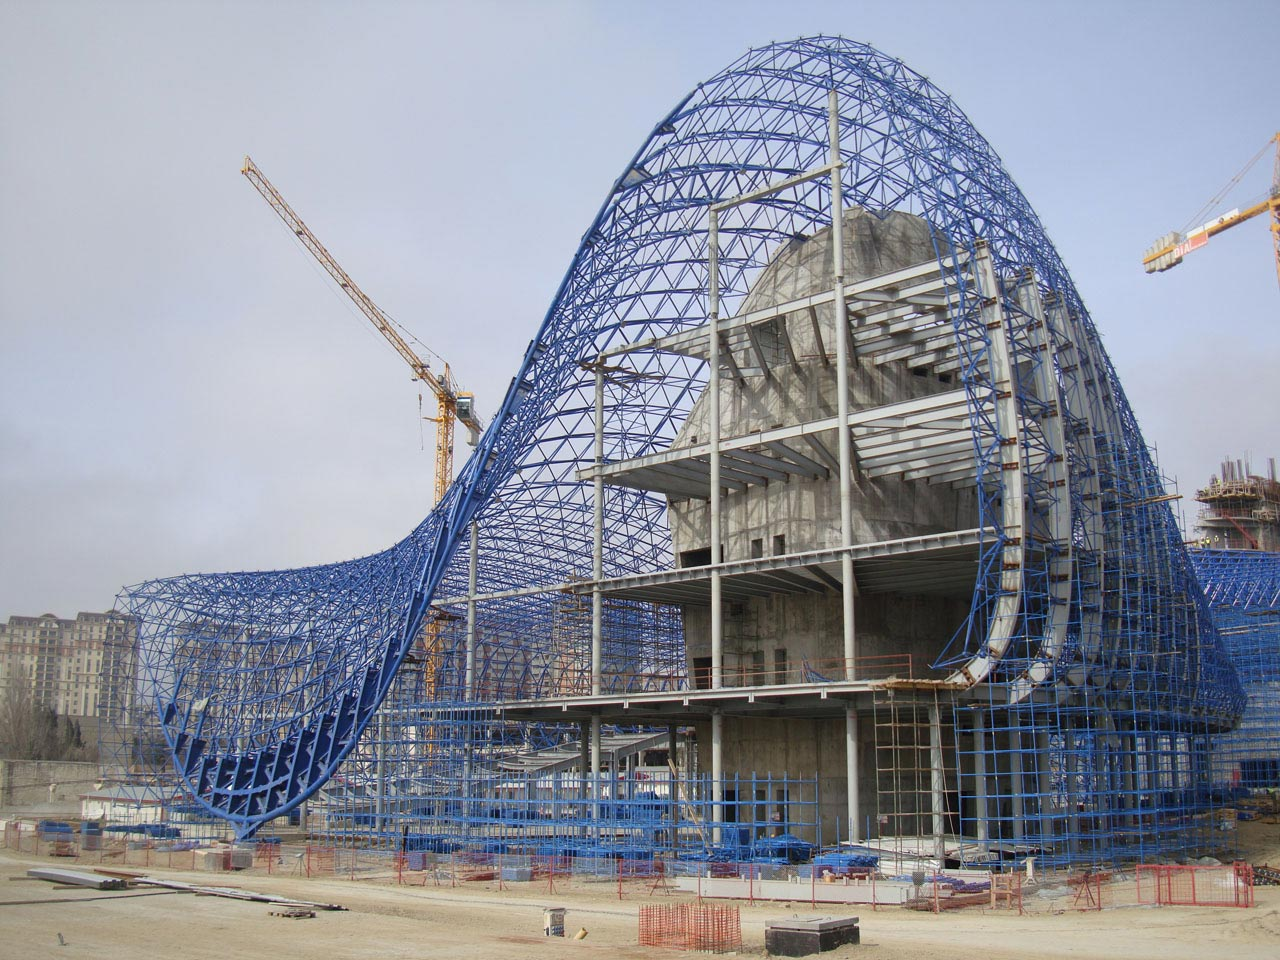
\includegraphics[ width = 0.7\textwidth]{Truss-other_05.jpg}
\end{figure}

\framebreak

\begin{figure}
\centering
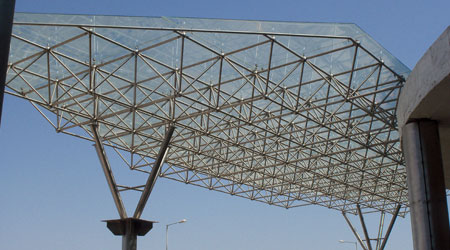
\includegraphics[ width = 0.7\textwidth]{Truss-other_03.jpg}
\end{figure}

\framebreak

\begin{figure}
\centering
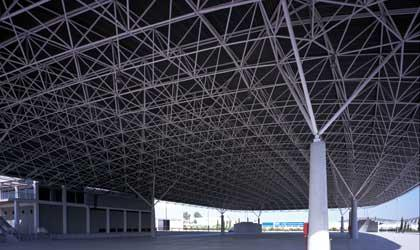
\includegraphics[ width = 0.7\textwidth]{Truss-other_02.jpg}
\end{figure}

\framebreak

\begin{figure}
\centering
\def\svgwidth{0.9\columnwidth}
\input{Fig_Vigas_Ejercicio_01.eps_tex}
\end{figure}

\end{frame}

% =============================================================================================
% =============================================================================================
\section{Componentes de una EVI}

% =============================================================================================
\subsection{Uniones Empernadas}

% =============================================================================================
\begin{frame}[allowframebreaks]
\frametitle{\insertsubsection}

\begin{figure}
\centering
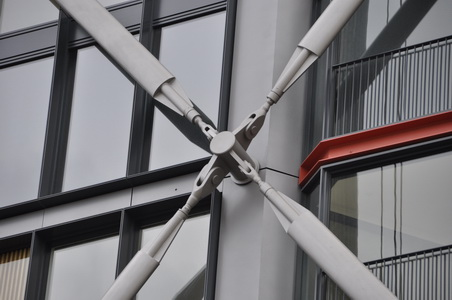
\includegraphics[ width = 0.8\textwidth]{Pinned-connection_02.jpg}
\end{figure}

\framebreak

\begin{figure}
\centering
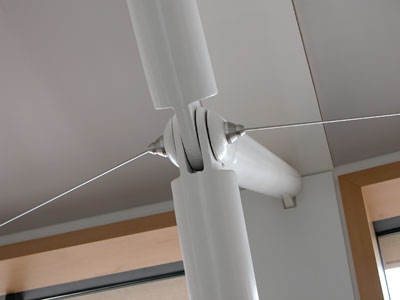
\includegraphics[ width = 0.7\textwidth]{Pinned-connection_03.jpg}
\end{figure}

\framebreak

\begin{figure}
\centering
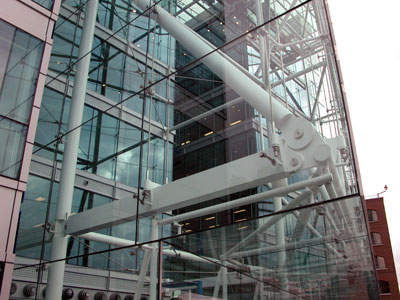
\includegraphics[ width = 0.7\textwidth]{Pinned-connection_04.jpg}
\end{figure}

\framebreak

\begin{figure}
\centering
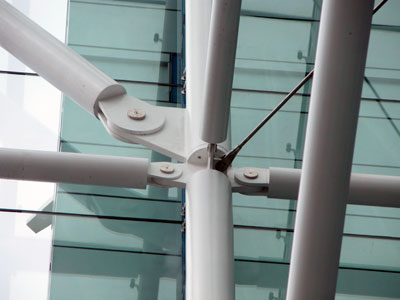
\includegraphics[ width = 0.7\textwidth]{Pinned-connection_05.jpg}
\end{figure}

\framebreak

\begin{figure}
\centering
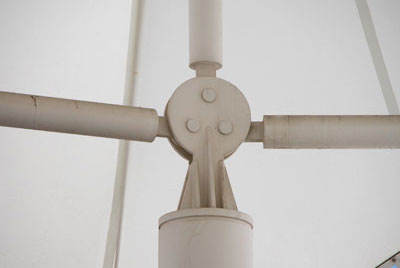
\includegraphics[ width = 0.7\textwidth]{Pinned-connection_07.jpg}
\end{figure}

%\framebreak
%
%\begin{figure}
%\centering
%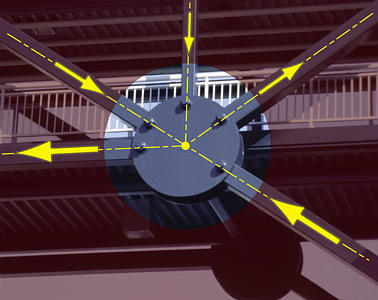
\includegraphics[ width = 0.64\textwidth]{Pinned-connection_08.jpeg}
%\end{figure}

\end{frame}

% =============================================================================================
\subsection{Soportes Empernados}

% =============================================================================================
\begin{frame}[allowframebreaks]
\frametitle{\insertsubsection}

\begin{figure}
\centering
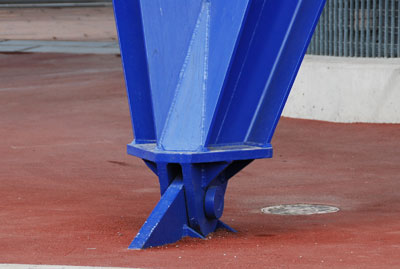
\includegraphics[ width = 0.8\textwidth]{Pinned-support_01.jpg}
\end{figure}

\framebreak

\begin{figure}
\centering
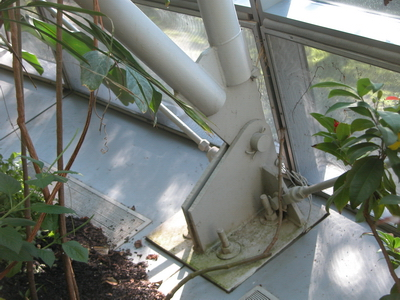
\includegraphics[ width = 0.7\textwidth]{Pinned-support_02.jpg}
\end{figure}

\framebreak

\begin{figure}
\centering
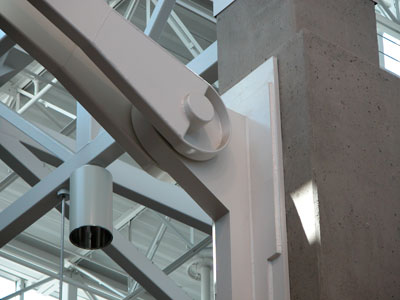
\includegraphics[ width = 0.7\textwidth]{Pinned-support_03.jpg}
\end{figure}

\framebreak

\begin{figure}
\centering
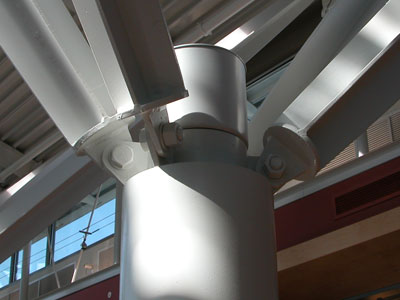
\includegraphics[ width = 0.8\textwidth]{Pinned-support_05.jpg}
\end{figure}

\framebreak

\begin{figure}
\centering
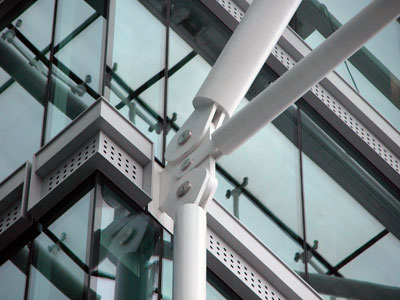
\includegraphics[ width = 0.7\textwidth]{Pinned-support_04.jpg}
\end{figure}

\end{frame}

% =============================================================================================
\subsection{Soportes Rodantes}

% =============================================================================================
\begin{frame}[allowframebreaks]
\frametitle{\insertsubsection}

\begin{figure}
\centering
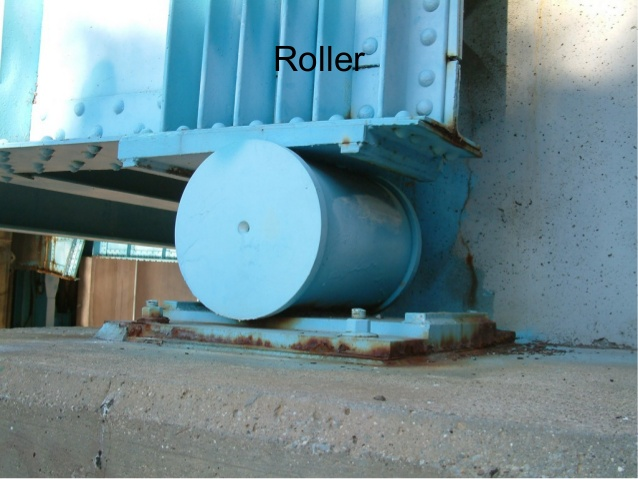
\includegraphics[ width = 0.7\textwidth]{Roller-support_01.jpg}
\end{figure}

\framebreak

\begin{figure}
\centering
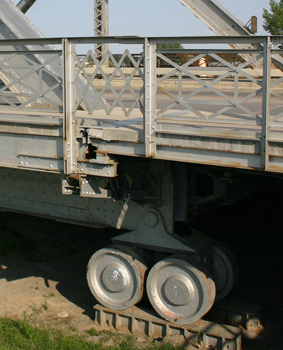
\includegraphics[ width = 0.5\textwidth]{Roller-support_02.jpg}
\end{figure}

\framebreak

\begin{figure}
\centering
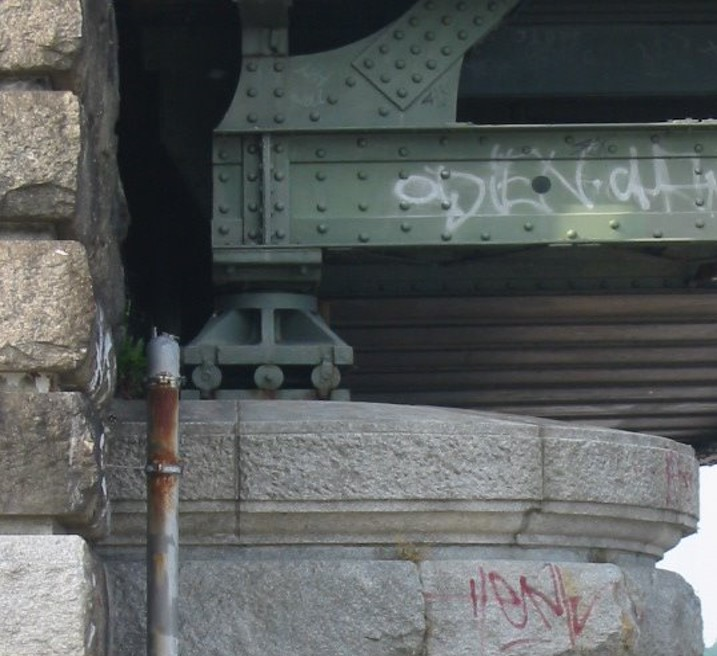
\includegraphics[ width = 0.6\textwidth]{Roller-support_04.jpg}
\end{figure}

\framebreak

\begin{figure}
\centering
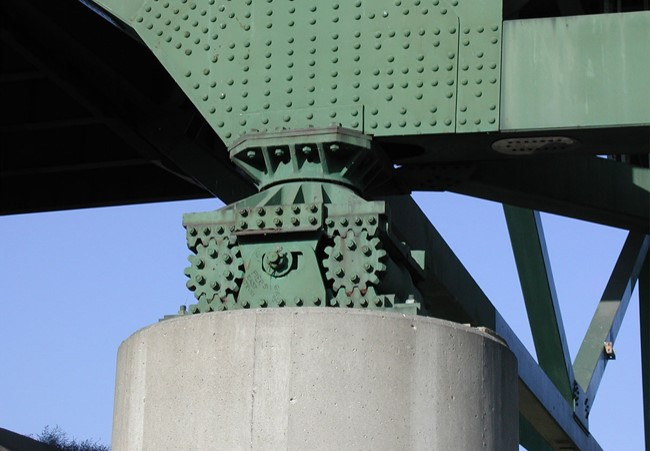
\includegraphics[ width = 0.8\textwidth]{Roller-support_06.jpg}
\end{figure}

\framebreak

\begin{figure}
\centering
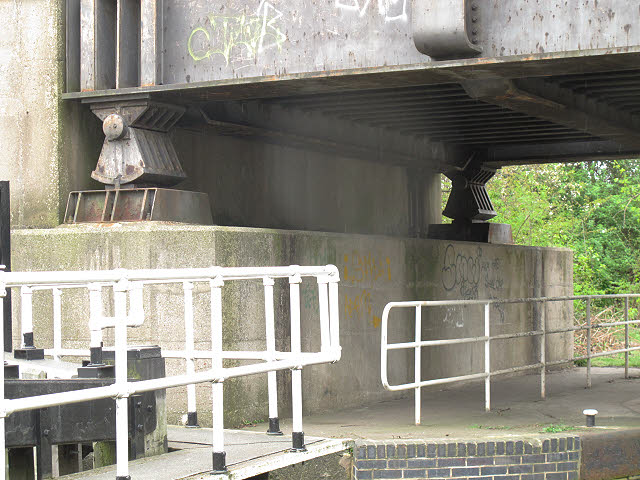
\includegraphics[ width = 0.7\textwidth]{Roller-support_05.jpg}
\end{figure}

\end{frame}

% =============================================================================================
% =============================================================================================
\section{M\'etodo de las Uniones para Analizar una EVI}

% =============================================================================================
\begin{frame}[allowframebreaks]
\frametitle{\insertsection}

\begin{figure}
\centering
\def\svgwidth{0.9\columnwidth}
\input{Fig_Vigas_Ejercicio_01.eps_tex}
\end{figure}

\framebreak

\begin{figure}
\centering
\def\svgwidth{0.9\columnwidth}
\input{Fig_Vigas_Ejercicio_01-Fuerzas.eps_tex}
\end{figure}

\framebreak

\begin{figure}
\centering
\def\svgwidth{0.9\columnwidth}
\input{Fig_Vigas_Ejercicio_02.eps_tex}
\end{figure}

\end{frame}

% =============================================================================================
\begin{frame}[allowframebreaks]
\frametitle{\insertsection}

\begin{itemize}
\item Nodo 1: 
\begin{align*}
& (x) \; -F_{12} - F_{15} \, \cos(45) + F_{13} \, \cos(45) = 0 \\
& (y) \; F_{14} + F_{13} \, \sin(45) + F_{15} \, \sin(45) = 0
\end{align*}
\item Nodo 2: 
\begin{align*}
& (x) \; F_{12} - F_{26} \, \cos(45) = 0 \\
& (y) \; F_{25} + F_{26} \, \sin(45) = 0
\end{align*}
\item Nodo 3: 
\begin{align*}
& (x) \; -F_{34} - F_{13} \, \cos(45) + T_3 = 0 \\
& (y) \; -F_{13} \, \sin(45) + N_3 = 0
\end{align*}
\framebreak
\item Nodo 4: 
\begin{align*}
& (x) \; F_{34} - F_{45} = 0 \\
& (y) \; -F_{14} = F_A
\end{align*}
\item Nodo 5: 
\begin{align*}
& (x) \; F_{15} \, \cos(45) + F_{45} - F_{56} = 0 \\
& (y) \; -F_{25} - F_{15} \, \sin(45) = F_B
\end{align*}
\item Nodo 6: 
\begin{align*}
& (x) \; F_{56} + F_{26} \, \cos(45) = 0 \\
& (y) \; -F_{26} \, \cos(45) + N_6 = 0
\end{align*}
\end{itemize}

\end{frame}

\end{document}
